\begin{qBox}{2}
Plot \( \langle E \rangle / N \) vs \( T \). 
Compare and discuss the results for the high and low temperature regimes.

\tcblower

Below shows the plot that I was able to produce: 

\begin{figure}[H]
    \centering
    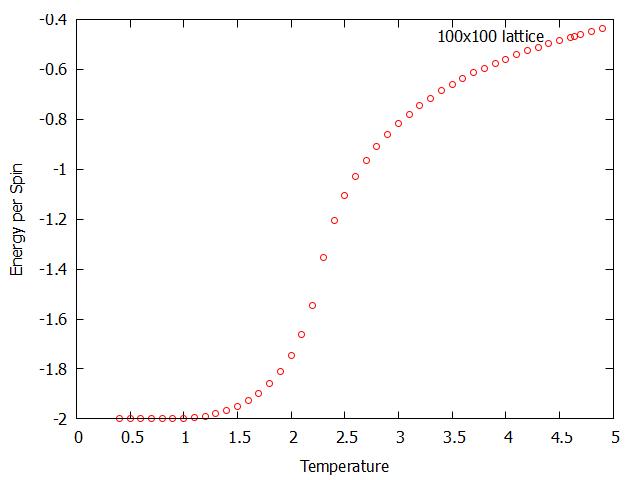
\includegraphics[ width = 0.5\linewidth ]{figures/assignment6_2.png}
    \caption{My plot for \( \langle E \rangle / N \) vs \( T \)}
\end{figure}

From this plot, we can see that the energy per spin at low temperatures is essentially
\( -2 \).
We expect this to be the case since the energy function of our system is given as 
follows (assuming no external magnetization -- i.e., \( H = 0 \)): 
\begin{equation*}
    E
    =
    - J \sum_{ \langle i j \rangle } s_{ i } s_{ j }
\end{equation*}
where the sum is over all pairs of nearest neighbor spin \( \langle i j \rangle \),
and \( J \) is the exchange constant that we are assuming to be positive. 
At lower temperatures, we expect these spins to mostly stay in the same direction.
Since we take each spin to have a magnitude of \( 1 \), we find that each particle 
has an energy contribution of \( 4 \) (one for each of its nearest neighbor),
which results in the sum to be the following:
\begin{equation*}
    T \text{ low}
    \implies 
    E = - J \sum_{ \langle i j \rangle } s_{ i } s_{ j } = - J \frac{ 4 N }{ 2 }
\end{equation*}
Note that we included the fact of \( 2 \) since we would be double counting the 
energy contributions otherwise.
Taking \( J = 1 \), results in the energy per spin to be \( -2 \).

\baseSkip 

Once the temperature starts increasing, we expect the energy to increase, which is 
what we do end up seeing in the plot.
Notice that we see the most rapid increase in energy per spin near the critical 
temperature, and we continue to see that energy increases (although at a lower rate)
as temperature further increases.
As noted in lecture, the energy does not tend to \( 0 \) as \( T \) increases to 
larger values, meaning that relative spin order must not be random.
\end{qBox}